
\begin{figure}[H]
    \centering
    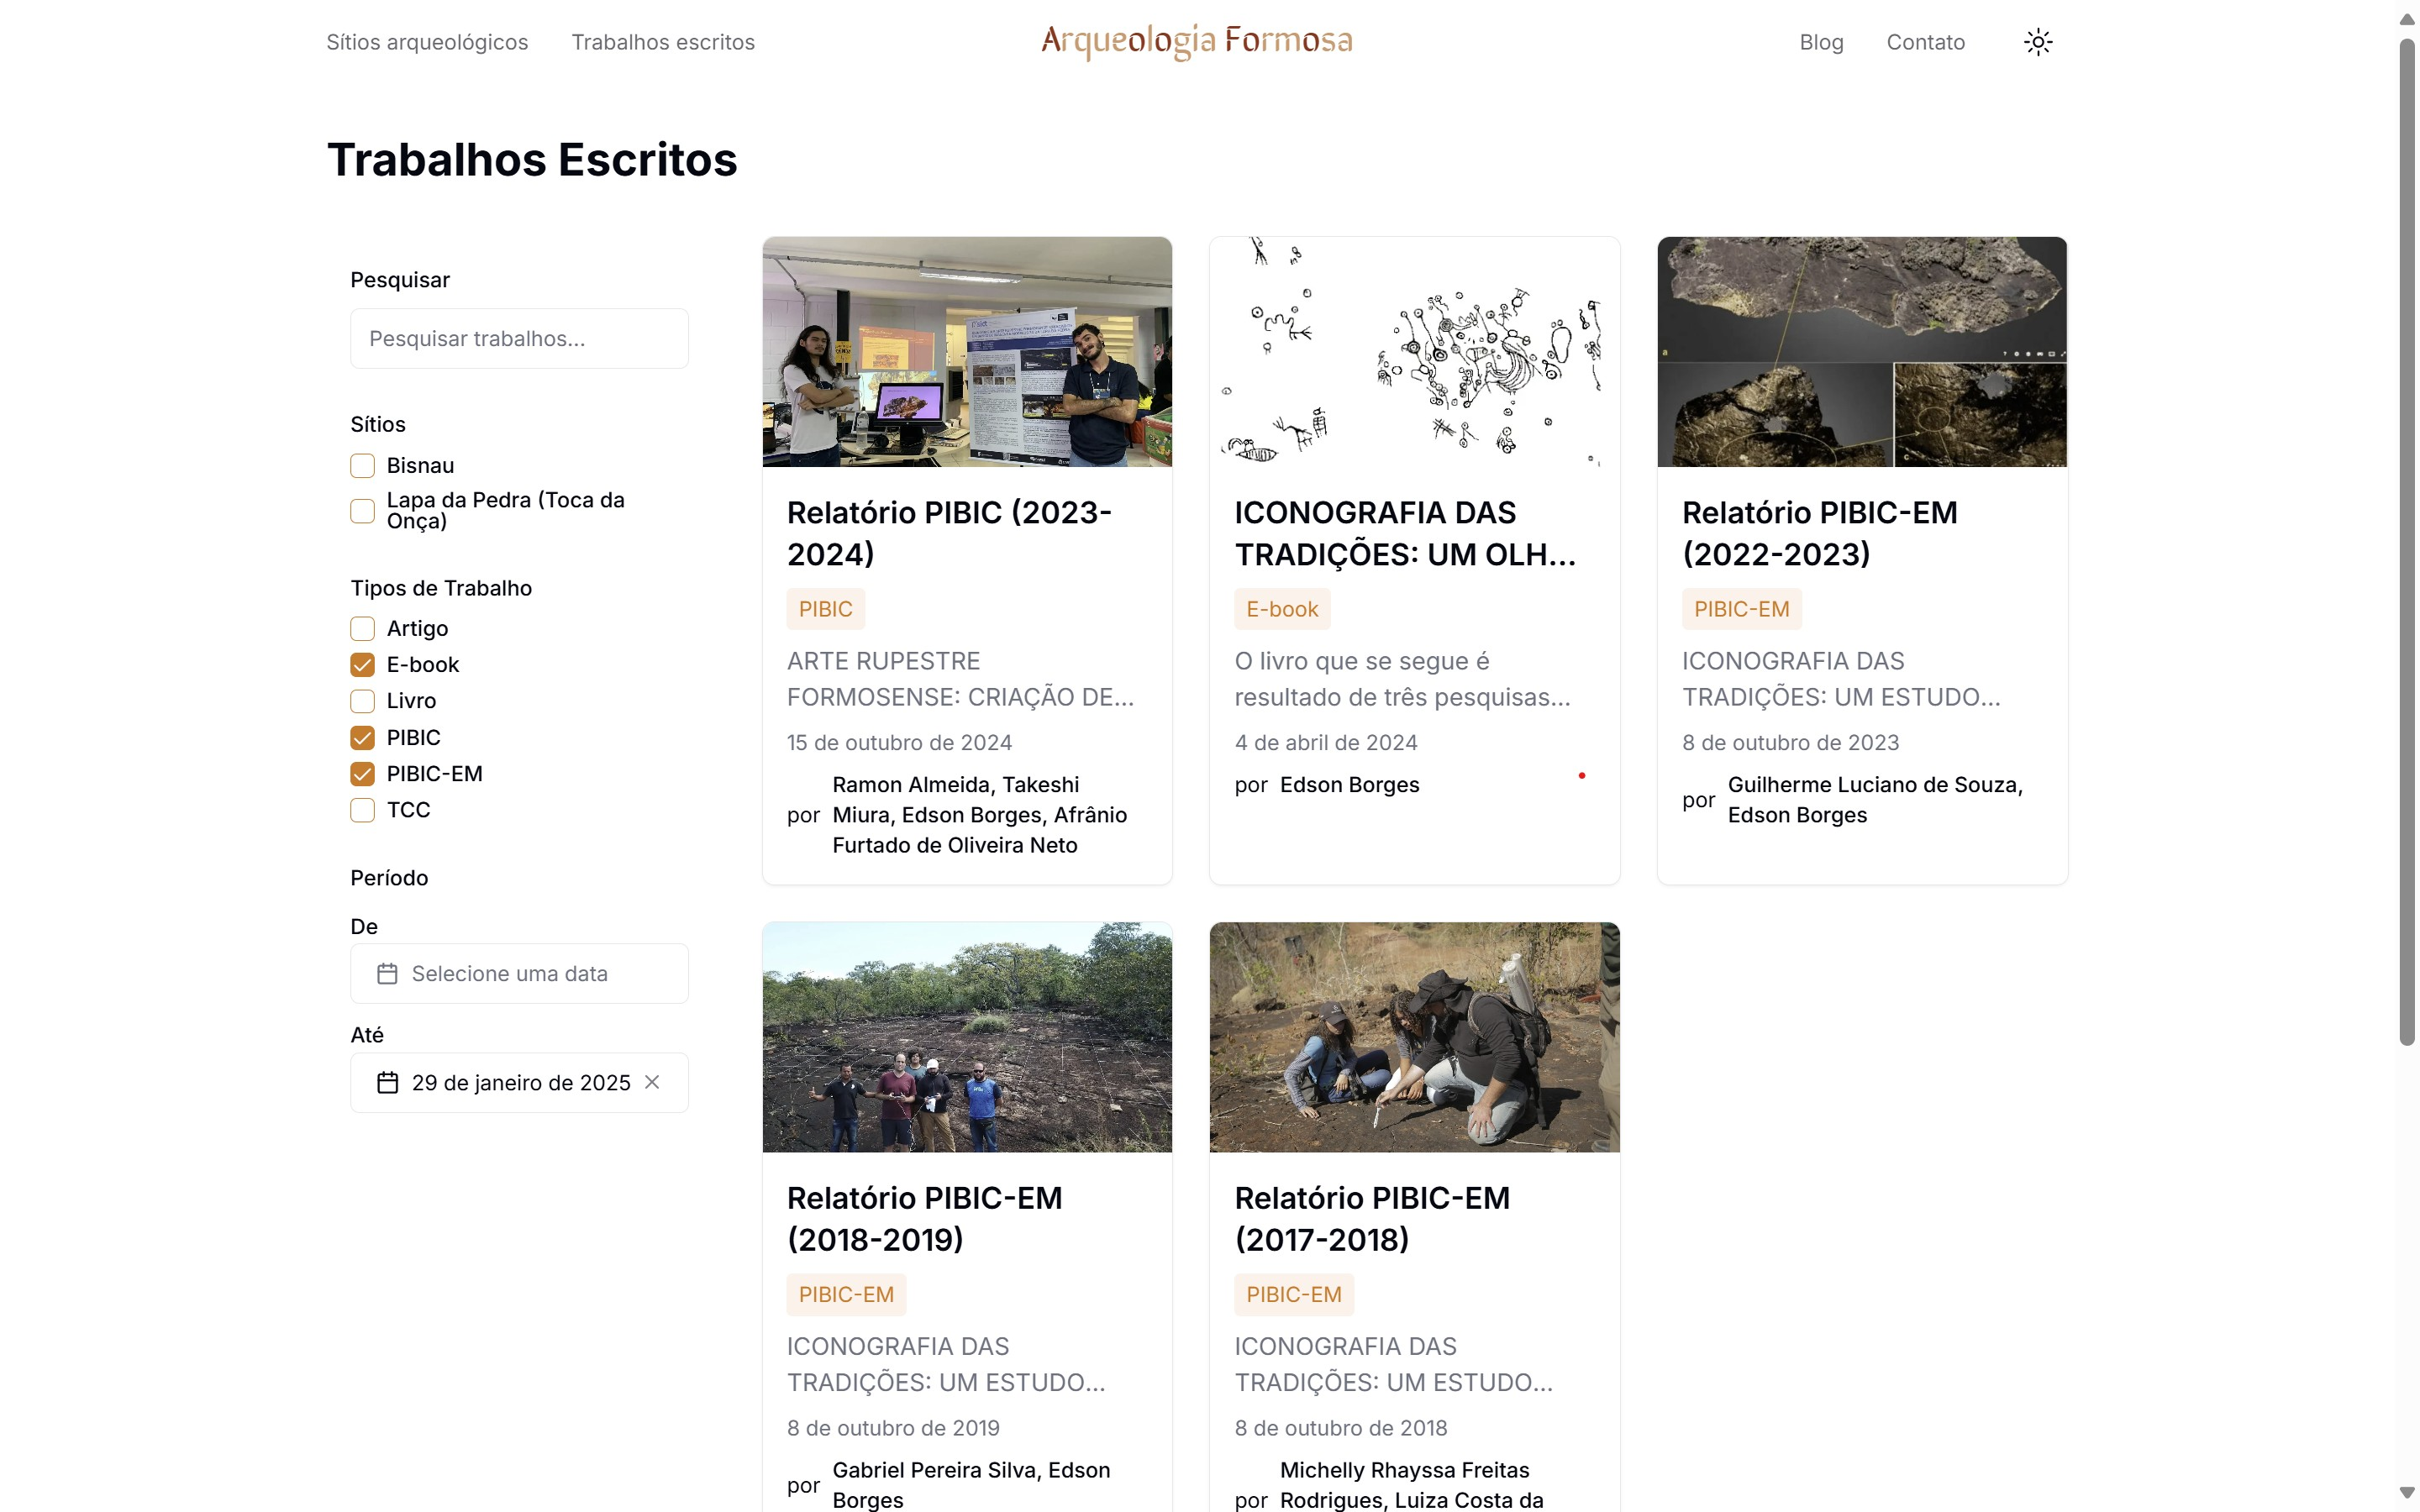
\includegraphics[height=10cm, keepaspectratio]{img/site/Trabalhos escritos.jpg}
    \caption{Página de Trabalhos escritos \\
    \textbf{Fonte:} Elaborado pelo autor, 2025.}
    \label{fig:pagina_trabalhos}
\end{figure}


\begin{figure}[H]
    \centering
    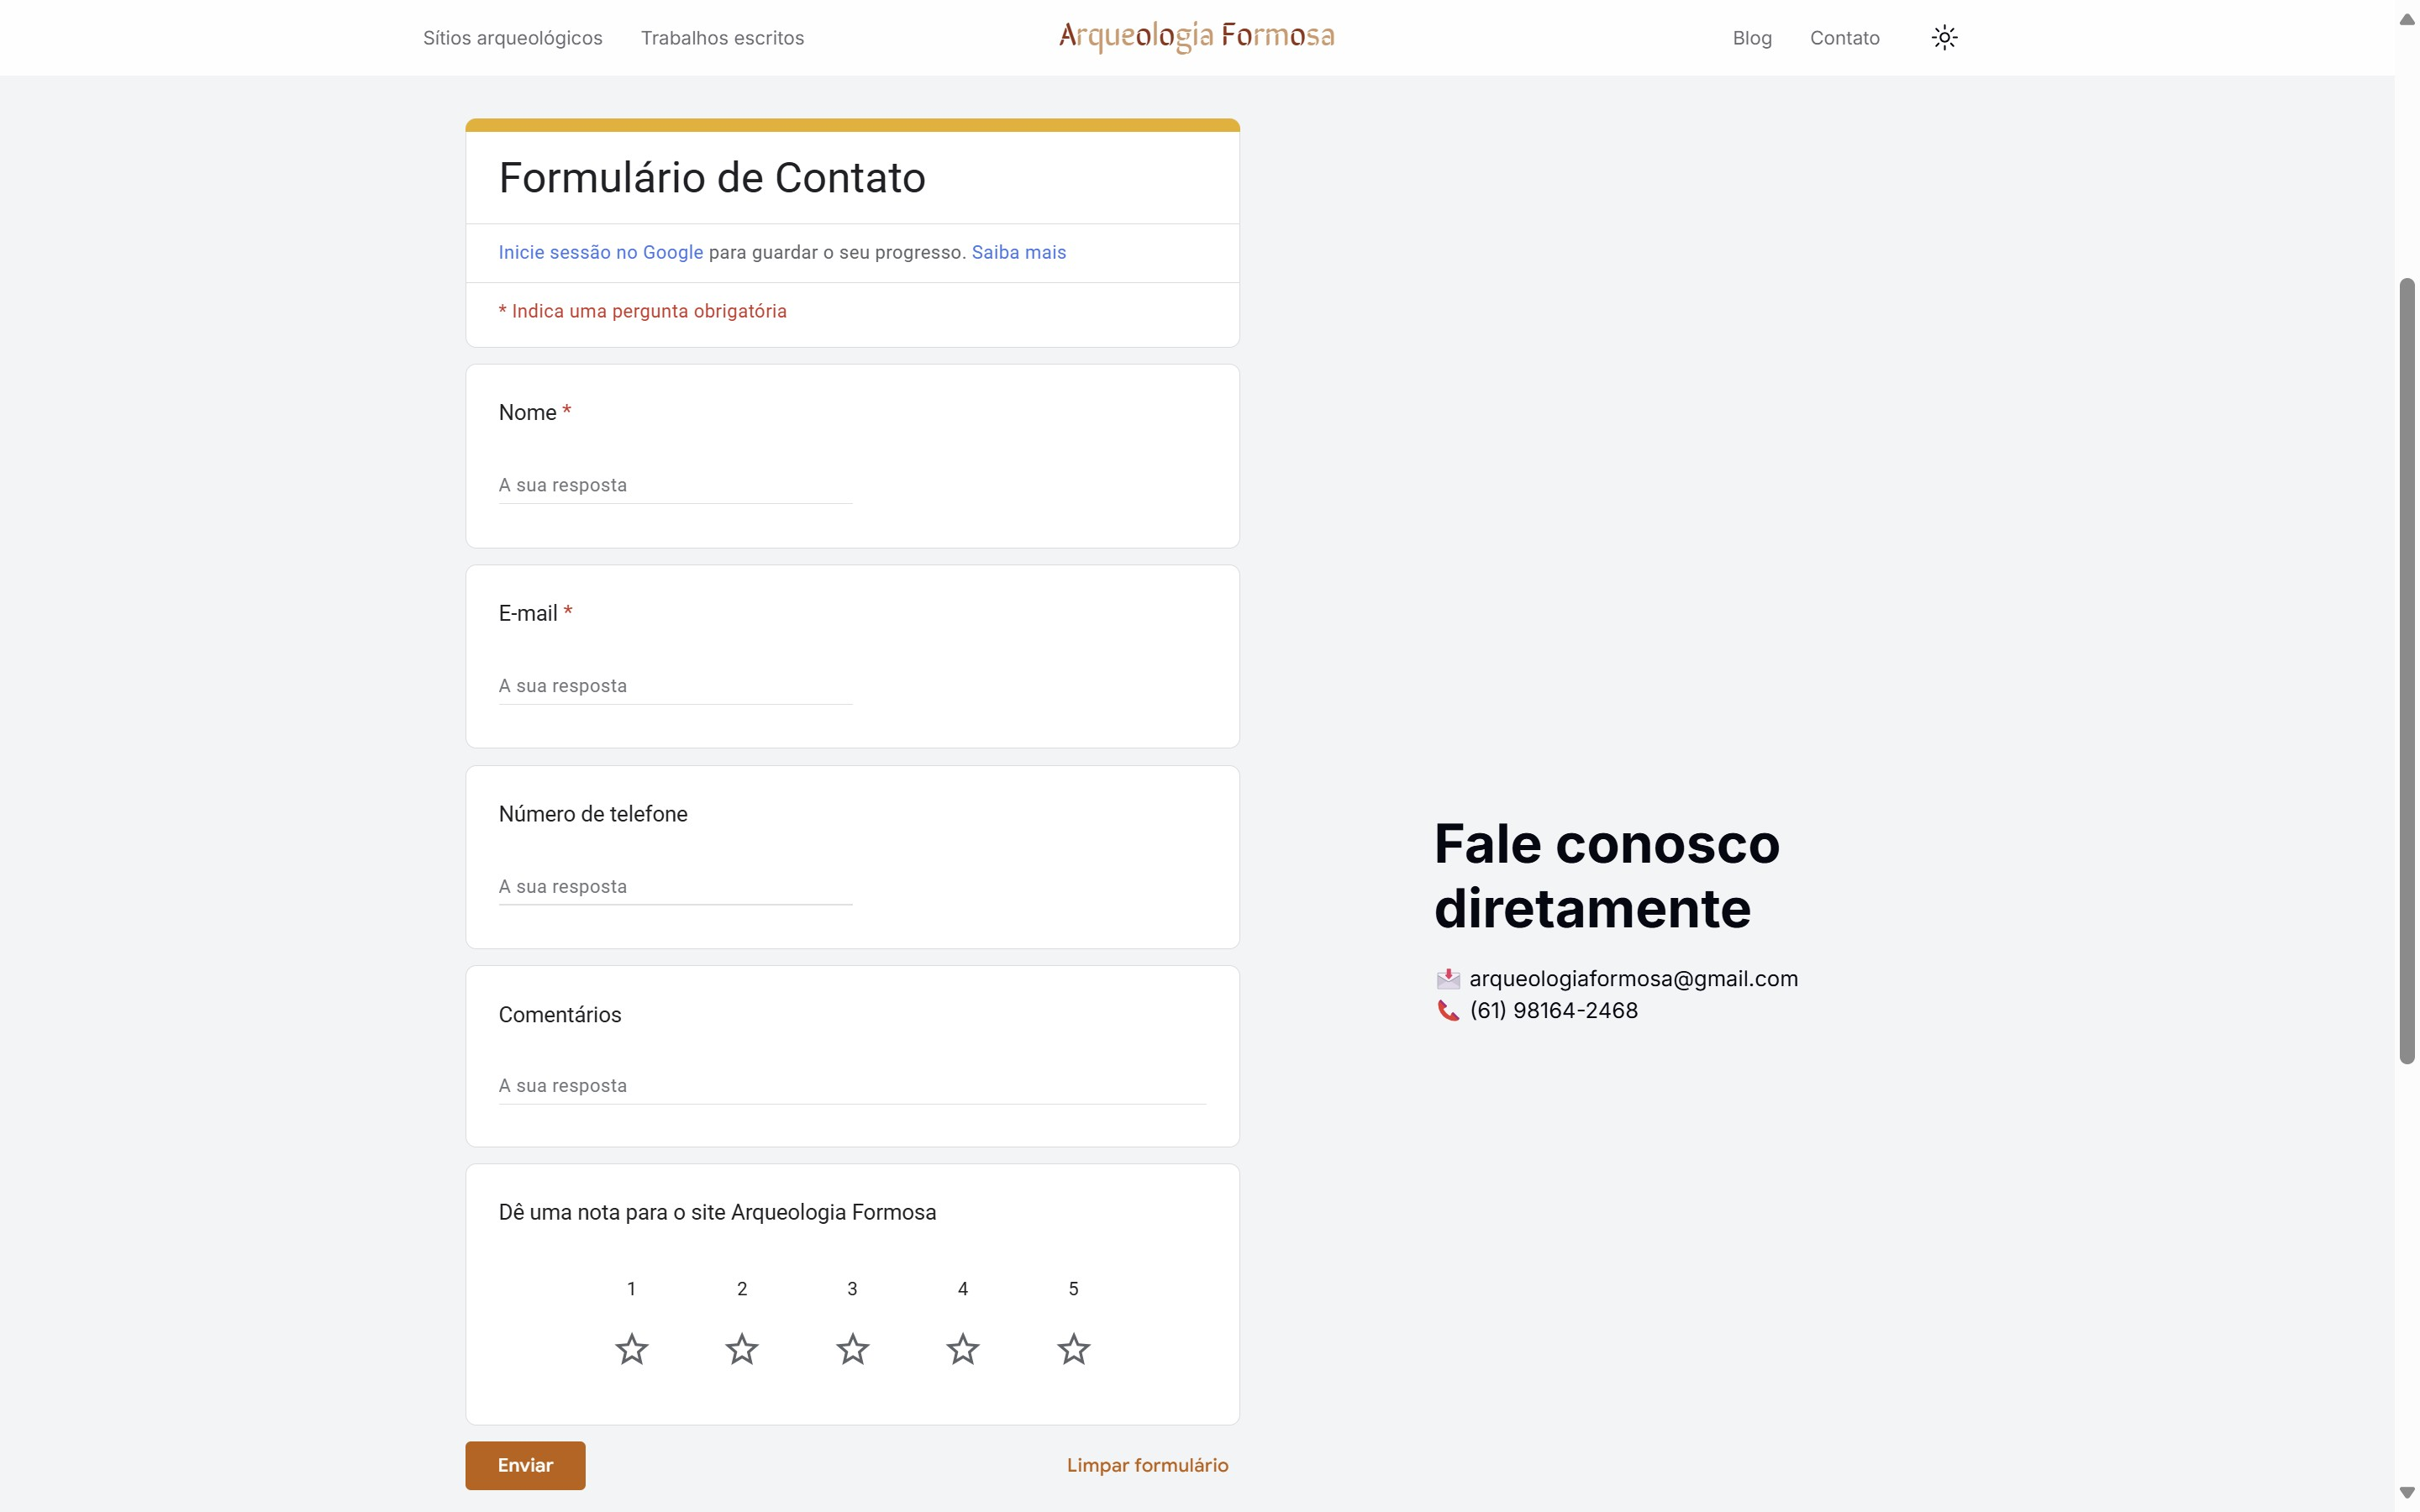
\includegraphics[height=10cm, keepaspectratio]{img/site/contato.jpg}
    \caption{Página de Contato \\
    \textbf{Fonte:} Elaborado pelo autor, 2025.}
    \label{fig:pagina_contato}
\end{figure}


\begin{figure}[H]
    \centering
    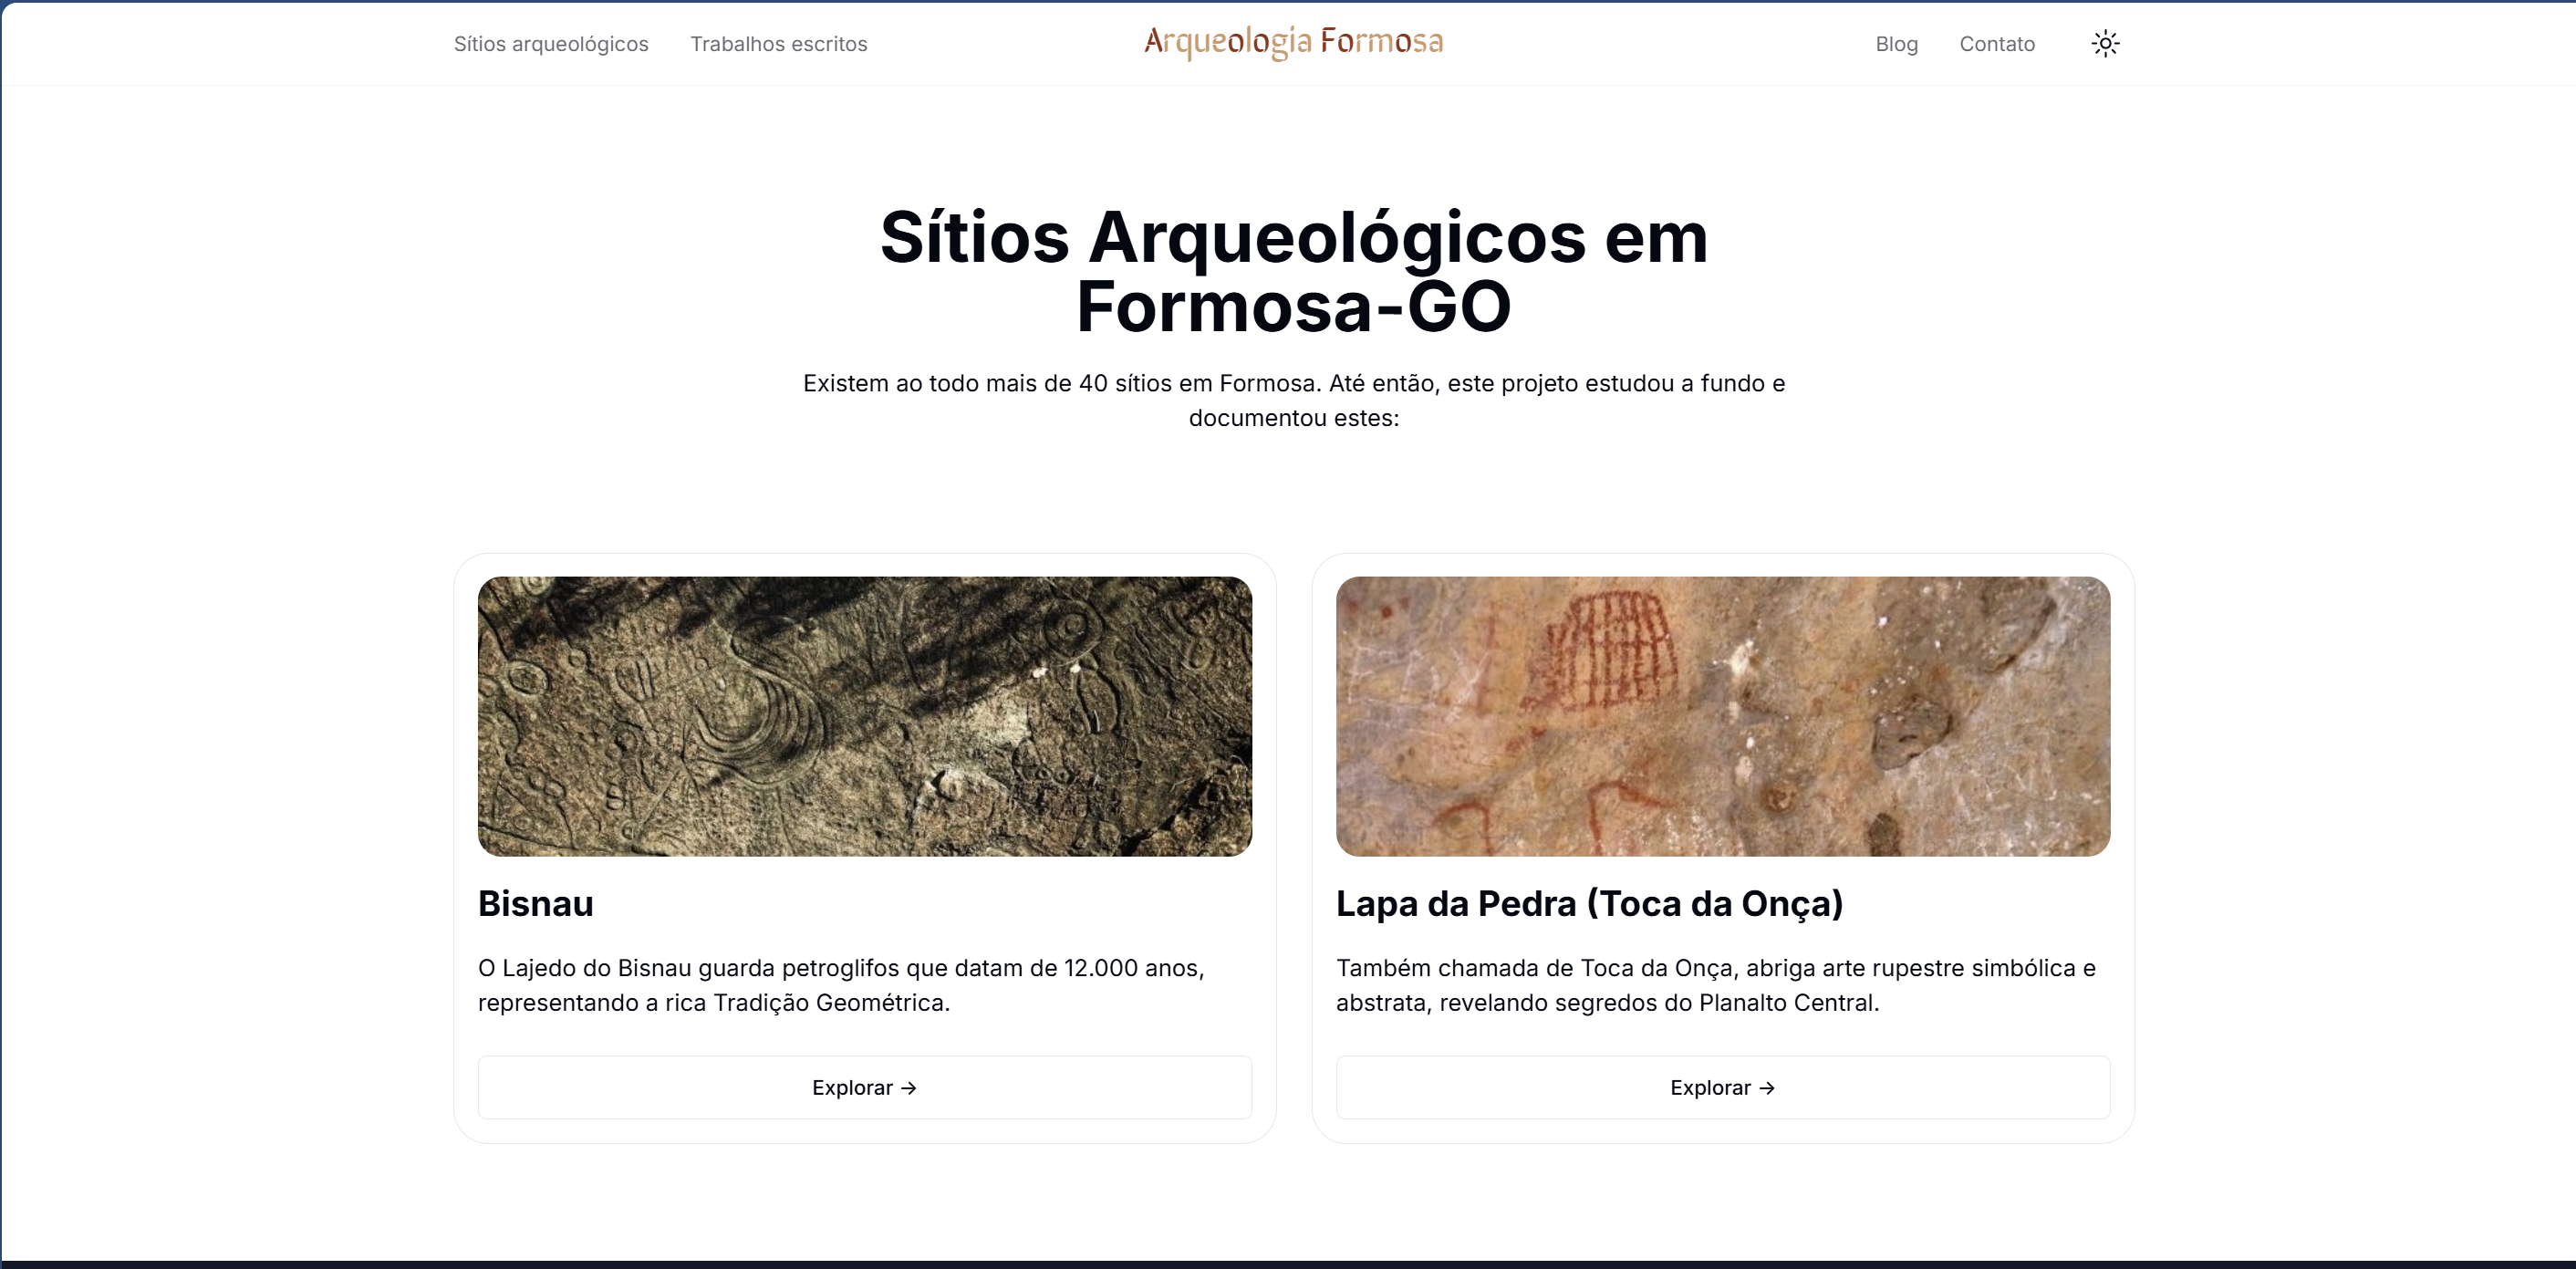
\includegraphics[height=8cm, keepaspectratio]{img/site/sitios arqueologicos.png}
    \caption{Página de Sítios Arqueológicos \\
    \textbf{Fonte:} Elaborado pelo autor, 2025.}
    \label{fig:pagina_sitiosarqueologicos}
\end{figure}

\begin{figure}[H]
    \centering
    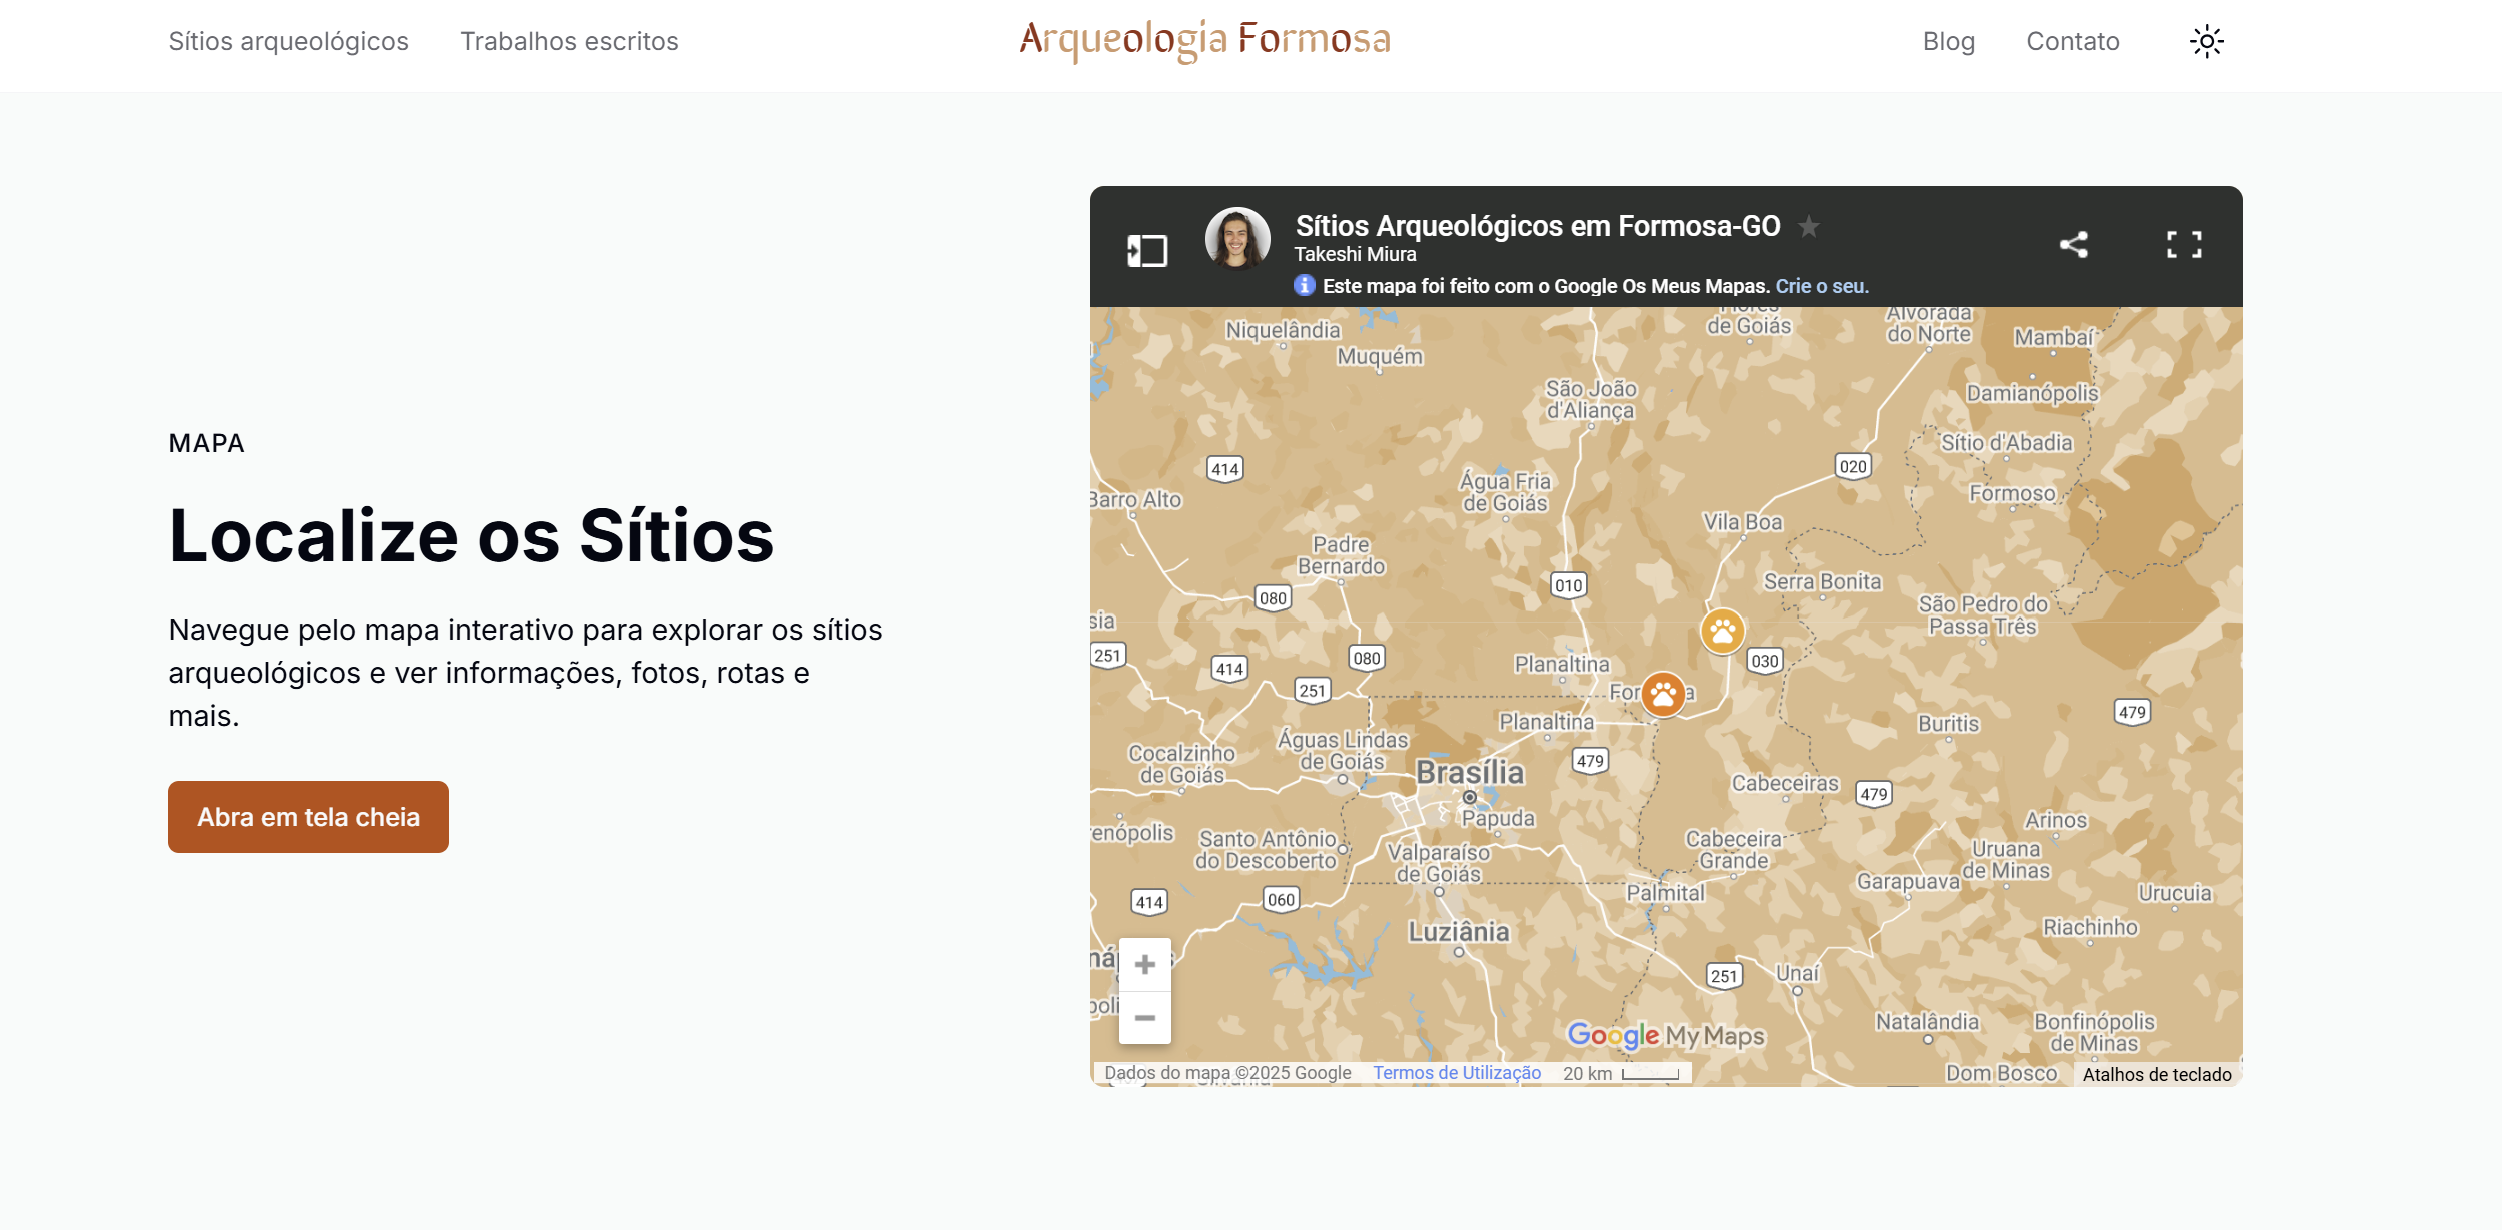
\includegraphics[height=8cm, keepaspectratio]{img/site/localize os sitios.png}
    \caption{ Mapa interativo com a localização dos sítios arqueológicos integrado ao site. \\
        \textbf{Fonte:} Elaborado pelo autor, 2025.}
    \label{fig:localize os sitios}
\end{figure}

\begin{figure}[H]
    \centering
    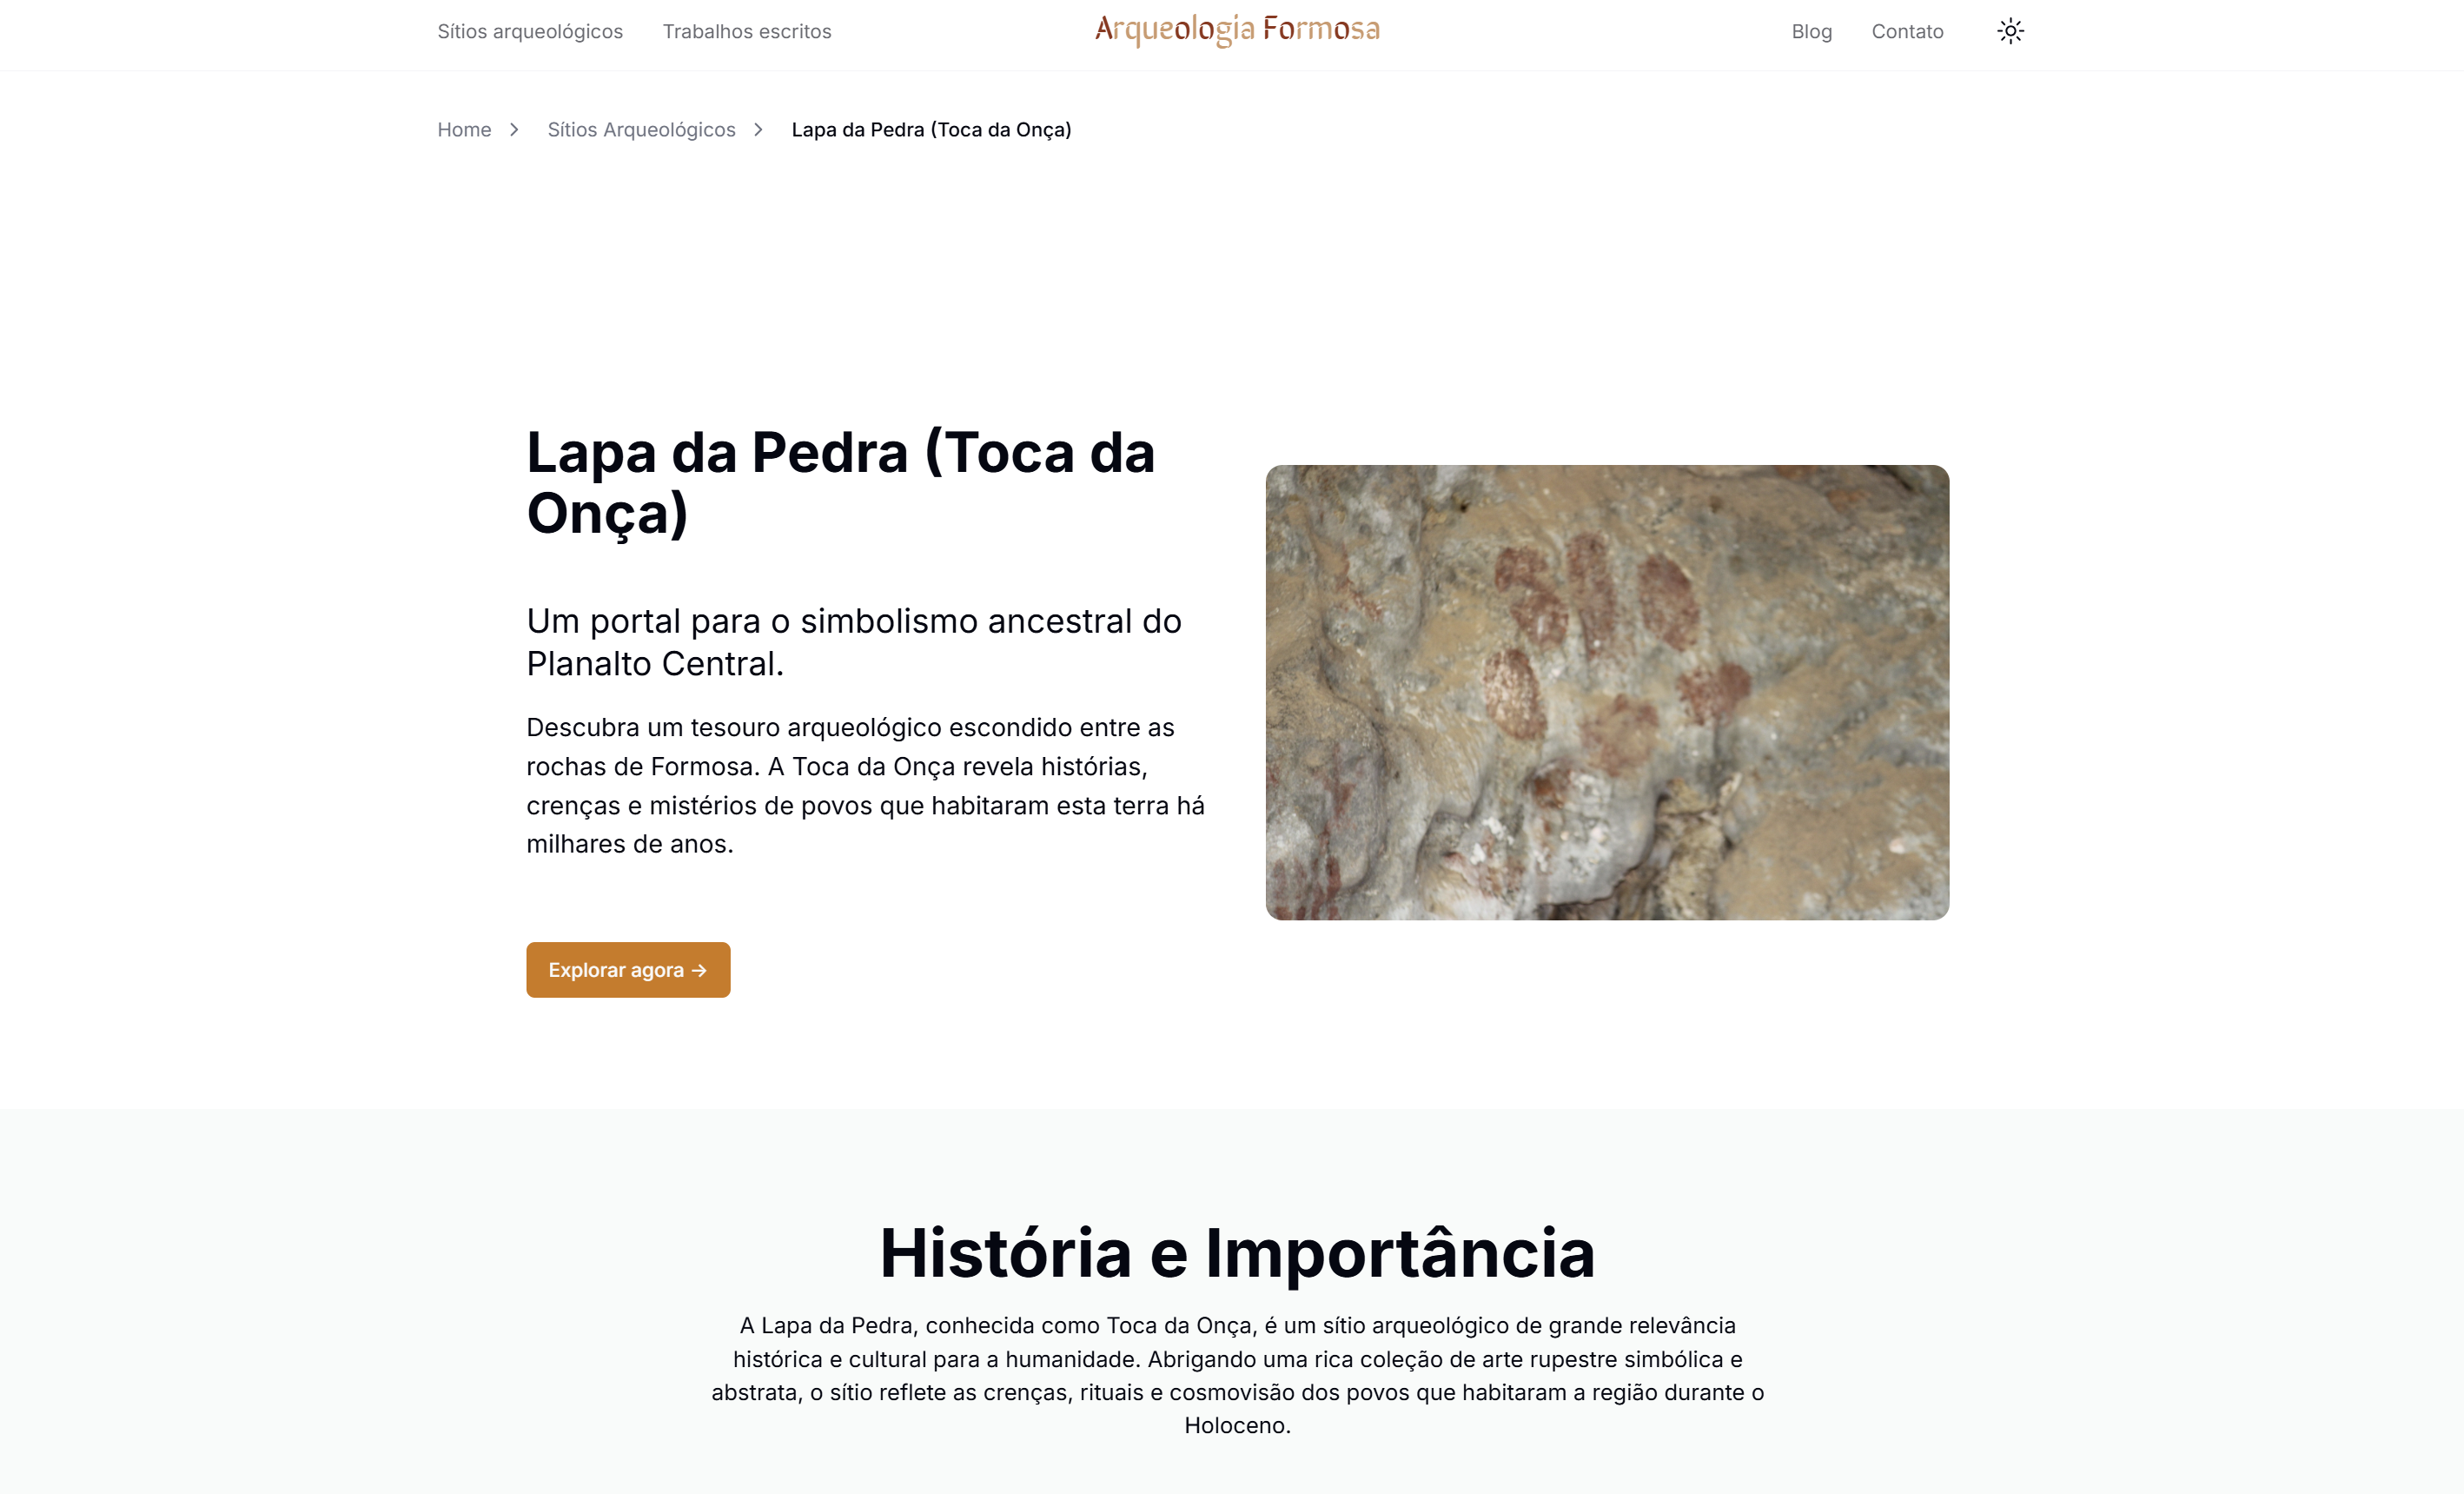
\includegraphics[height=10cm, keepaspectratio]{img/site/pagina_toca_da_onca.png}
    \caption{Página do Sítio Toca da Onça \\
    \textbf{Fonte:} Elaborado pelo autor, 2025.}
    \label{fig:pagina_tocadaonca}
\end{figure}

\begin{figure}[H]
    \centering
    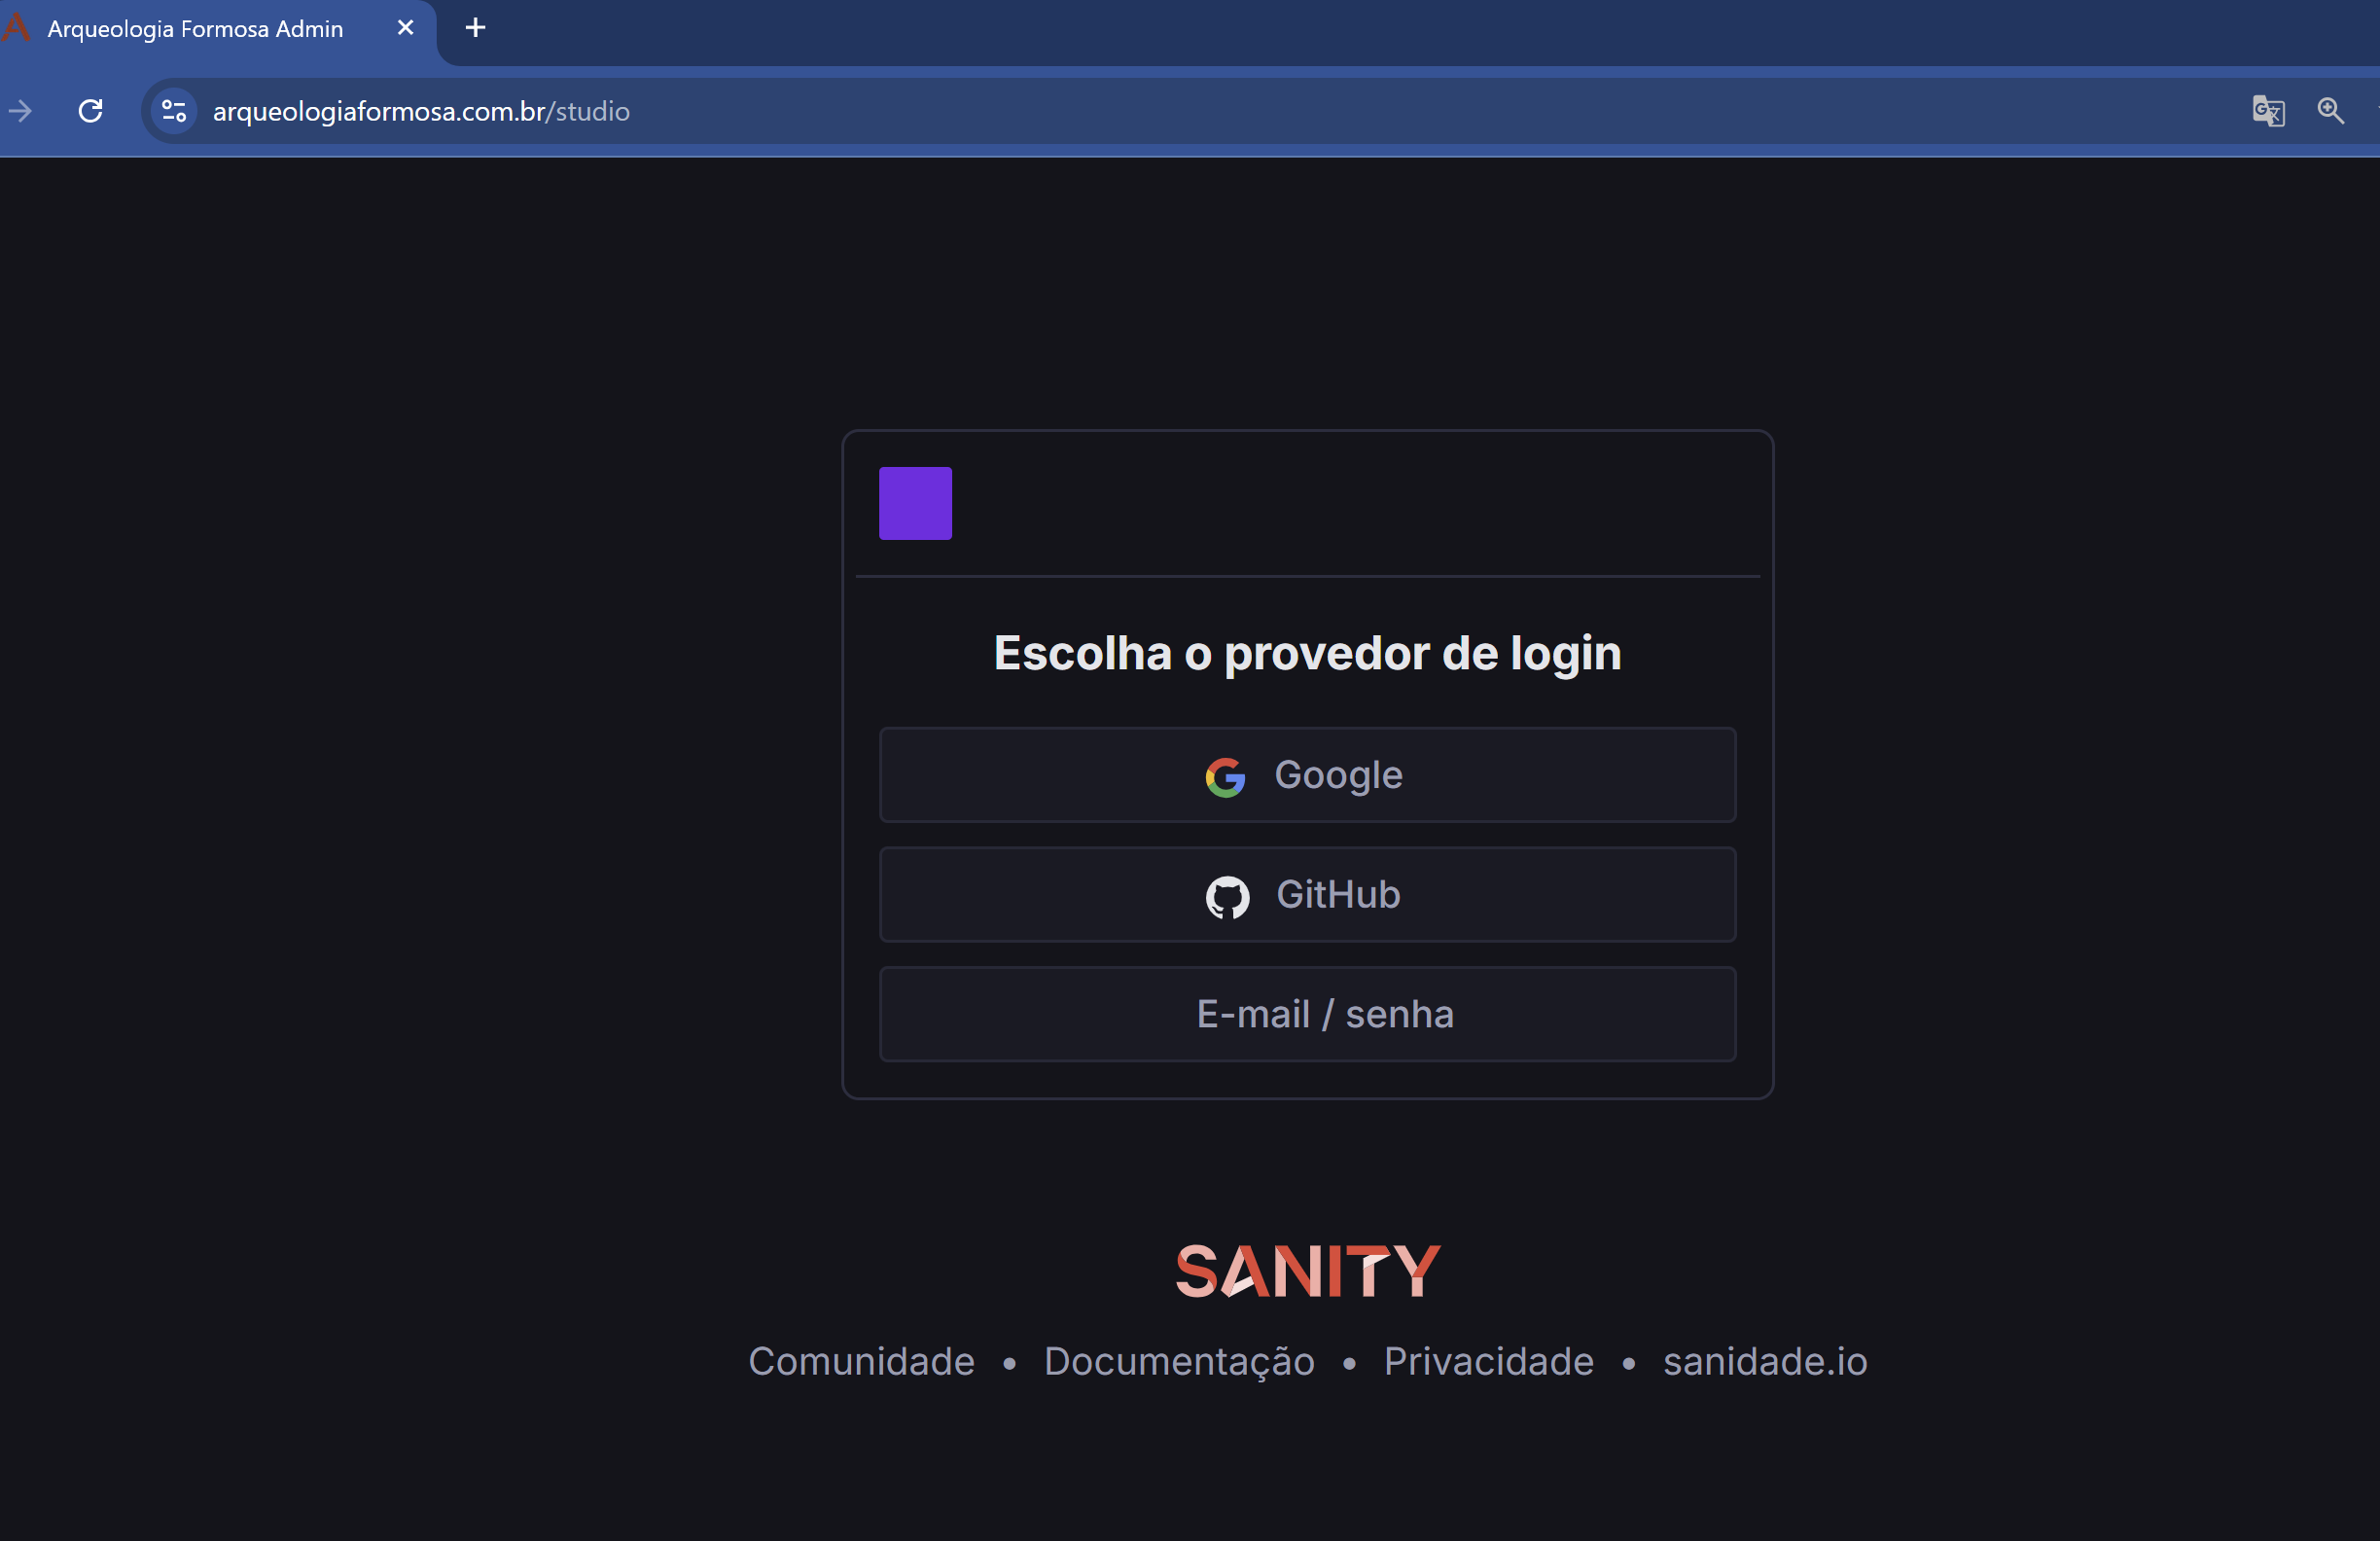
\includegraphics[height=3cm, keepaspectratio]{img/site/login.png}
    \caption{Página de Login para acesso da área administrativa. \\
    \textbf{Fonte:} Elaborado pelo autor, 2025.}
    \label{fig:footer}
\end{figure}

                    \begin{figure}[H]
                        \centering
                        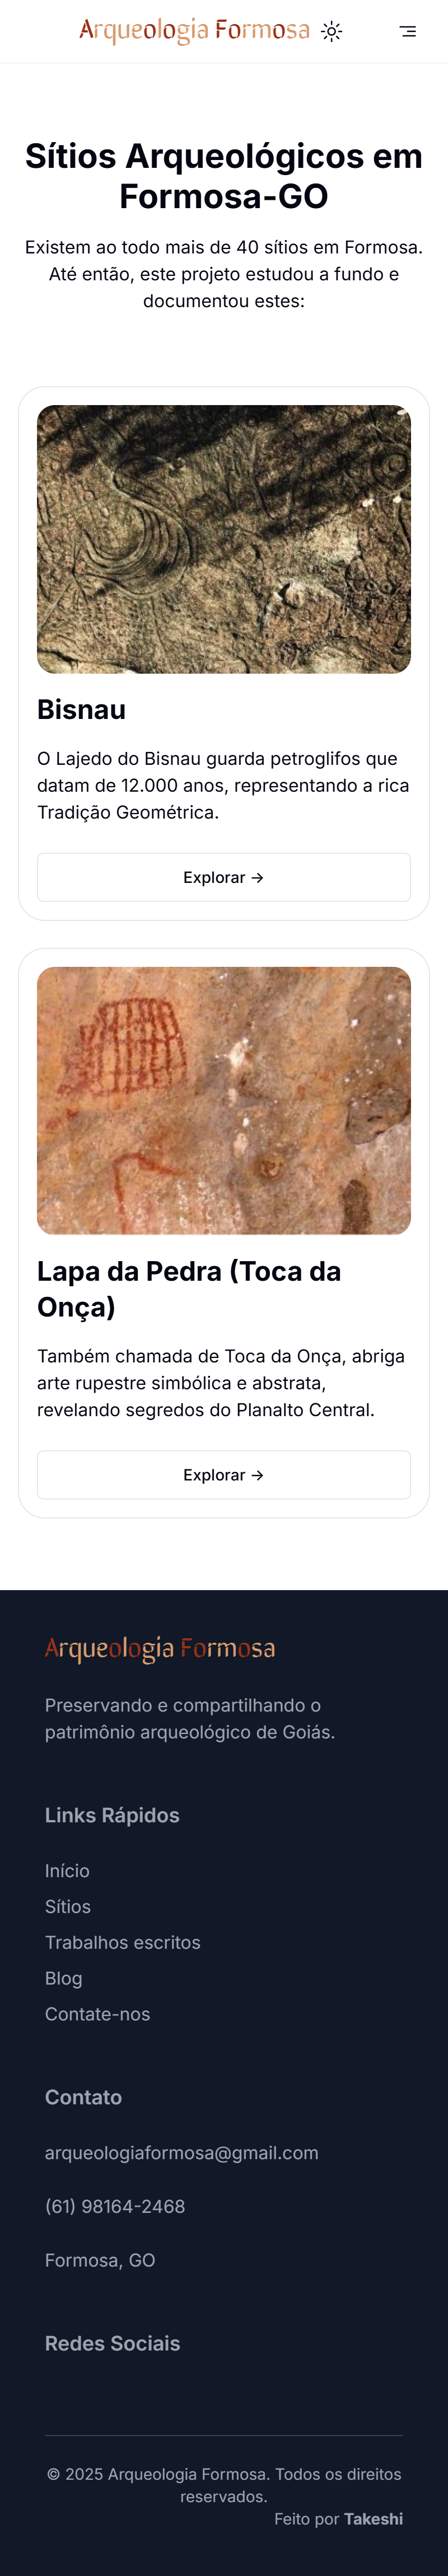
\includegraphics[height=22cm, keepaspectratio]{img/site/site mobile.png}
                        \caption{ Interdace responsiva para dispositivos móveis.  \\
                            \textbf{Fonte:} Elaborado pelo autor, 2025.}
                        \label{fig:responsivo1}
                    \end{figure}

\begin{figure}[H]
    \centering
    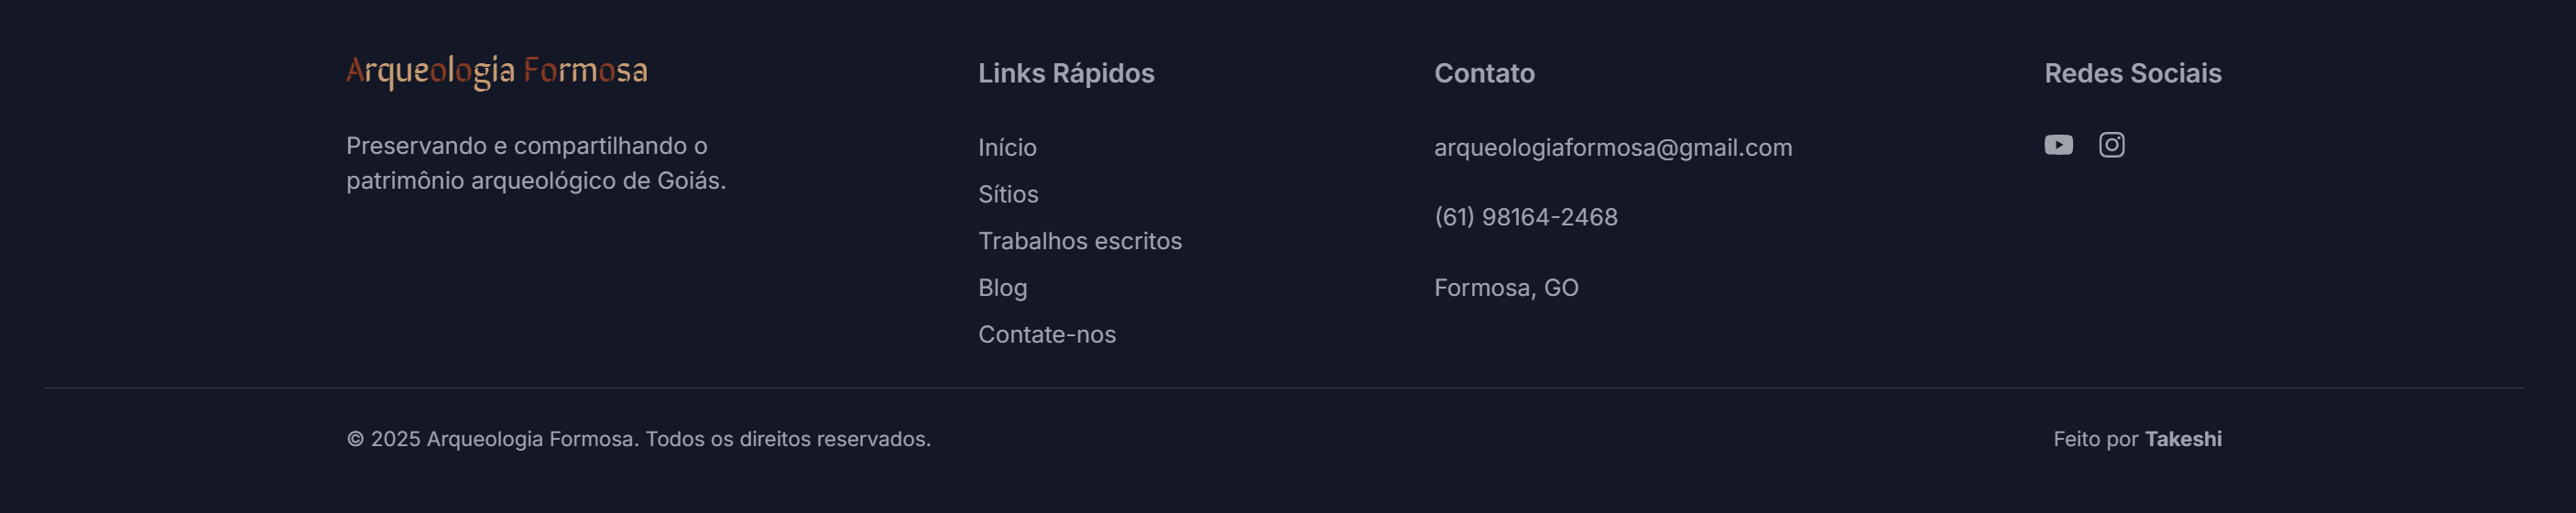
\includegraphics[height=3cm, keepaspectratio]{img/site/footer.png}
    \caption{Rodapé do Site Arqueologia Formosa. \\
    \textbf{Fonte:} Elaborado pelo autor, 2025.}
    \label{fig:footer}
\end{figure}

